\lhead{\begin{tikzpicture}[remember picture, overlay]
    \node [anchor=100,inner sep=0] (imagenIZQUIERDA) at (current page header area.north){
\includegraphics[width=18cm]{img/Encabezado.PNG}};
    \end{tikzpicture}}
    \rhead{Ángeles-Hurtado}
    \rfoot{\begin{tikzpicture}[remember picture, overlay]
    \node [anchor=140,inner sep=0] (imagenDERECHA) at (current page footer area.south){
\includegraphics[width=18cm]{img/Foot.PNG}};
    \end{tikzpicture}}
    %----------------------------------------------------------------------------------------
    \lfoot{ \thepage}
    % \renewcommand{\labelenumi}{\alph{enumi}.)} 
    %----------------------------------------------------------------------------------------
    %----------------------------------------------------------------------------------------
    %	TITLE SECTION
    %----------------------------------------------------------------------------------------
    
    \setlength{\droptitle}{-5\baselineskip} % Move the title up
    \title{\textbf{Estudio de tiempos y movimientos en el ensamble de un circuito electrónico utilizando diferentes métodos para su optimización }} % Article title
    
     \author{ 
     \textsc{Rangel Frias Valeria}\\ 
    %  Afiliación:
     \texttt{ Instituto Tecnologico De Queretaro } \\ 
     \texttt{Tecnologico Nacional de Mexico } \\ 
     \texttt{Queretaro, Mexico}\\ 
     \texttt{Correo} 
     \and 
     \textsc{Ángeles-Hurtado, Luis Alberto}\\ 
    %  Afiliación:
     \texttt{ Instituto Tecnológico de Querétaro } \\ 
     \texttt{ Tecnológico Nacional de México } \\ 
     \texttt{Querétaro, México}\\ 
     \texttt{alb3rt0.ah@gmail.com} 
    }
    
    
    %----------------------------------------------------------------------------------------
    
    % \begin{document}
    
    % Print the title
    \maketitle
    \thispagestyle{fancy}
    
    %----------------------------------------------------------------------------------------
    %	ARTICLE CONTENTS
    %----------------------------------------------------------------------------------------
    
    % \section*{Resumen}
    % \textit{Palabras clave:}
    % El resumen (ancho de página) deberá contener entre 100 y 200 palabras tipo Adobe Devangari 11 puntos.
    
    \begin{abstract}
    \noindent 
    El resumen (ancho de página) deberá contener entre 100 y 200 palabras tipo Adobe Devangari 11 puntos.
    
    \end{abstract}
    % 
    % 
    \textbf{\textit{Palabras clave}}: {First keyword should be the corresponding to the research area according with the authors guide. Maximum of 6 keywords.}
    % \keywords{First keyword should be the corresponding to the research area according with the authors guide. Maximum of 6 keywords.}
    
    \section{Introducción}
    
    % Define estudio de tiempos y movimientos 
    El estudio de tiempos y movimientos es una técnica que tiene por objeto, en el ámbito del trabajo, evitar movimientos innecesarios del trabajador que sólo sirven para que el tiempo de cada operación sea mayor.
    
    Sus objetivos son reducir, lo más posible, el tiempo necesario para ejecutar cada trabajo, minimizar costes conservando los recursos, mejorar la calidad y confianza en el producto eliminando o reduciendo los movimientos ineficientes y acelerando los eficientes.
    
    % define que es ensamble
    
    Un proceso de ensamble implica la colocación de dos o más piezas individuales para la conformación de un producto final. Suele dividirse en niveles dependiendo de la cantidad de componentes a unir, ya sean mecánicos, de software, electrónicos, farmacéuticos, o de cualquier otro tipo.
    % define que es circuito electronico
    
    Un circuito electrónico consiste en una estructura de placas formadas por materiales semiconductores, materiales activos y pasivos, cuyo funcionamiento es crear un recorrido completo por el cual pueda viajar la corriente.
    
    % define el metodo de tiempos predeterminados
    
    Los tiempos predeterminados, son una reunión de tiempos estándares válidos asignados a movimientos fundamentales y grupos de movimientos que no pueden ser evaluados de forma precisa con los procedimientos ordinarios para estudio de tiempos con cronómetro.
    
    % define optimización
    
    La optimización es la acción de desarrollar una actividad lo más eficientemente posible, es decir, con la menor cantidad de recursos y en el menor tiempo posible. Es decir, la optimización significa realizar una tarea de la mejor manera, pudiéndose aplicar a distintos ámbitos. La optimización, en general, implica lograr el mejor funcionamiento de algo, usando de la mejor forma los recursos.
    % \begin{itemize}
    
    % \end{itemize}
    % 
    % 
    \section{Justificación}
    El estudio de tiempos y movimientos en el ensamble de un circuito electrónico es fundamental para garantizar eficiencia, calidad y productividad en la producción. La optimización de estos procesos a través de diferentes métodos proporciona ventajas significativas para las empresas, desde la reducción de costos hasta la mejora en la satisfacción del cliente.
    Un estudio de tiempos y movimientos permite identificar y eliminar operaciones innecesarias o redundantes en el ensamble del circuito electrónico.
    Reducción de Costos
    La optimización de los tiempos y movimientos conlleva una reducción en los costos operativos. Al eliminar desperdicios y mejorar la eficiencia, las empresas pueden reducir los costos de mano de obra, energía y materiales.
    Mejora en la Calidad
    Un ensamble eficiente y bien organizado reduce la probabilidad de errores y defectos en los circuitos electrónicos. Los métodos de estudio de tiempos y movimientos permiten identificar puntos críticos donde pueden ocurrir errores y establecer controles de calidad más efectivos.
    Conclusión
    En resumen, el estudio de tiempos y movimientos en el ensamble de un circuito electrónico utilizando diferentes métodos para su optimización es una herramienta invaluable para las empresas que buscan mejorar su competitividad en el mercado. Proporciona beneficios tangibles como la eficiencia en la producción, la reducción de costos, la mejora en la calidad, la flexibilidad y la innovación. Por lo tanto, invertir en este tipo de estudios es esencial para asegurar el éxito a largo plazo y el crecimiento sostenible de la empresa en la industria electrónica.
    \begin{itemize}
        \item 
    \end{itemize}
    % 
    % 
    \section{Descripción del problema}
    En el estudio de tiempos y movimientos en un ensamble de un circuito electrico es un problema que puede manifestarse de diversas formas y tener múltiples causas, pero sus consecuencias suelen ser perjudiciales para la operación de la línea de producción y para la satisfacción del cliente. A continuación, se describe con más detalle este problema y sus implicaciones:
    Movimientos Innecesarios
    Los movimientos innecesarios se refieren a acciones que no añaden valor al proceso de ensamble del circuito electrónico.
    Ineficiencia en los Movimientos
    La ineficiencia en los movimientos se manifiesta cuando los operadores realizan tareas de manera subóptima, utilizando más tiempo o esfuerzo del necesario. Esto puede ser causado por una falta de entrenamiento adecuado, herramientas inadecuadas, o un diseño deficiente de los puestos de trabajo.
    Impacto en la Calidad
    Los movimientos innecesarios pueden llevar a errores y defectos en el ensamble del circuito electrónico. 
    Costos Operativos Elevados
    La presencia de movimientos innecesarios e ineficientes incrementa los costos operativos al consumir más recursos, como mano de obra, tiempo y energía. Esto puede afectar la rentabilidad de la empresa y su capacidad para competir en el mercado.
    \begin{itemize}
        \item 
    \end{itemize}
    
    \textbf{*La incógnita científica es el elemento cuya solución incrementa el conocimiento científico.}
    % 
    % 
    \section{Fundamentación teórica}
    el estudio de tiempos y movimientos en el ensamble de circuitos electrónicos desempeña un papel fundamental en la optimización de los procesos de producción. La fundamentación teórica basada en la Teoría de los Tiempos y Movimientos, la ergonomía, el enfoque Lean Manufacturing, la calidad y la mejora continua, así como la incorporación de tecnologías avanzadas, respalda la importancia de esta disciplina para mejorar la eficiencia, la productividad y la calidad del producto final en la industria electrónica.
    \begin{itemize}
        \item 
    \end{itemize}
    % 
    % 
    \section{Hipótesis}
    La complejidad inherente al proceso de ensamble de un circuito eléctrico conlleva desafíos específicos que afectan la eficiencia, la productividad y la calidad del producto final. Sin embargo, mediante la aplicación de técnicas avanzadas de estudio de tiempos y movimientos, así como la incorporación de tecnologías y prácticas de mejora continua, es posible optimizar el proceso de ensamble, superar los desafíos identificados y mejorar significativamente los indicadores de desempeño del proceso
    Desafíos Identificados
    Los desafíos identificados en el proceso de ensamble pueden incluir movimientos innecesarios, tiempos de ciclo prolongados, dificultades ergonómicas, riesgos de daño a los componentes electrónicos, variabilidad en la calidad del producto y dificultades para adaptarse a cambios en la demanda del mercado o en los requisitos del producto.
    Verificación de la Hipótesis:
    Para verificar la hipótesis, se pueden llevar a cabo las siguientes acciones:Estudio Detallado del Proceso,Aplicación de Técnicas de Estudio de Tiempos y Movimientos,Incorporación de Tecnologías y Prácticas de Mejora Continua,Evaluación de Resultados,Validación de la Hipótesis
    
    \begin{itemize}
        \item 
    \end{itemize}
    % 
    % 
    \section{Objetivo}
    probar la hipótesis planteada para este proyecto de ensamble de circuito eléctrico que integre métodos de estudio de tiempos y movimientos, herramientas etc para la optimización  y mejora en el proceso de ensamblaje 
    
    \begin{itemize}
        \item
    \end{itemize}
    
    \subsection{Objetivos específicos }
    Los objetivos específicos en la elaboración de un estudio de tiempos y movimientos en el ensamble de un circuito electrónico se centran en identificar, analizar y optimizar los procesos de producción para mejorar la eficiencia, la productividad y la calidad del producto final. Al utilizar diferentes métodos y técnicas, se busca abordar los desafíos y complejidades inherentes al proceso de ensamble, implementando mejoras que contribuyan al éxito y la competitividad de las empresas en la industria electrónica.
    ALGUNOS DE ELLOS SON:
    IDENTIFICAR MOVIMIENTOS INNECESARIOS , MEDIR TIEMPOS DE OPERACIÓN,ANALIZAR EL FLUJO DE TRABAJO, OPTIMIZAR LA DISTRIBUCIÓN DE ESTACIONES DE TRABAJO, IMPLEMENTAR MEJORAS ERGONÓMICAS .
    
    \begin{itemize}
        \item 
    \end{itemize}
    
    % 
    % 
    \section{Cuerpo (Metodología, modelo matemático, etc.)}
    
    Cada estrategia metodológica se establece acorde a cada objetivo, y por tanto deberá ser desglosada precisada y ordenada claramente. En consecuencia cada objetivo que se presentó en forma de verbo en infinitivo deberá determinar una estrategia en forma de adverbio. Ej. Desarrollar…Desarrollo. Son las actividades ordenadas que tienen como finalidad la prueba de la hipótesis. 
    
    \begin{itemize}
        \item Se debe establecer que se habrá de hacer, como, conque, y donde para obtener la información que permita probar la hipótesis.  
        \item Se debe desglosar de acuerdo a los objetivos específicos. 
        \item Se debe establecer una estrategia metodológica por cada objetivo específico. De manera simplista se podría decir que se cambia el verbo en infinitivo por su respectivo adverbio.
        \item En cada objetivo se debe describir que método, que materiales y que equipo se usará para conseguirlo.
        \item Se deben tener referencias Figura \ref{fig:lcd-16x2-1}.
        VEASE EL APENDICE \ref{anexo:1}
    \end{itemize}
    % 
    % 
    \begin{figure}[H]
        \centering
        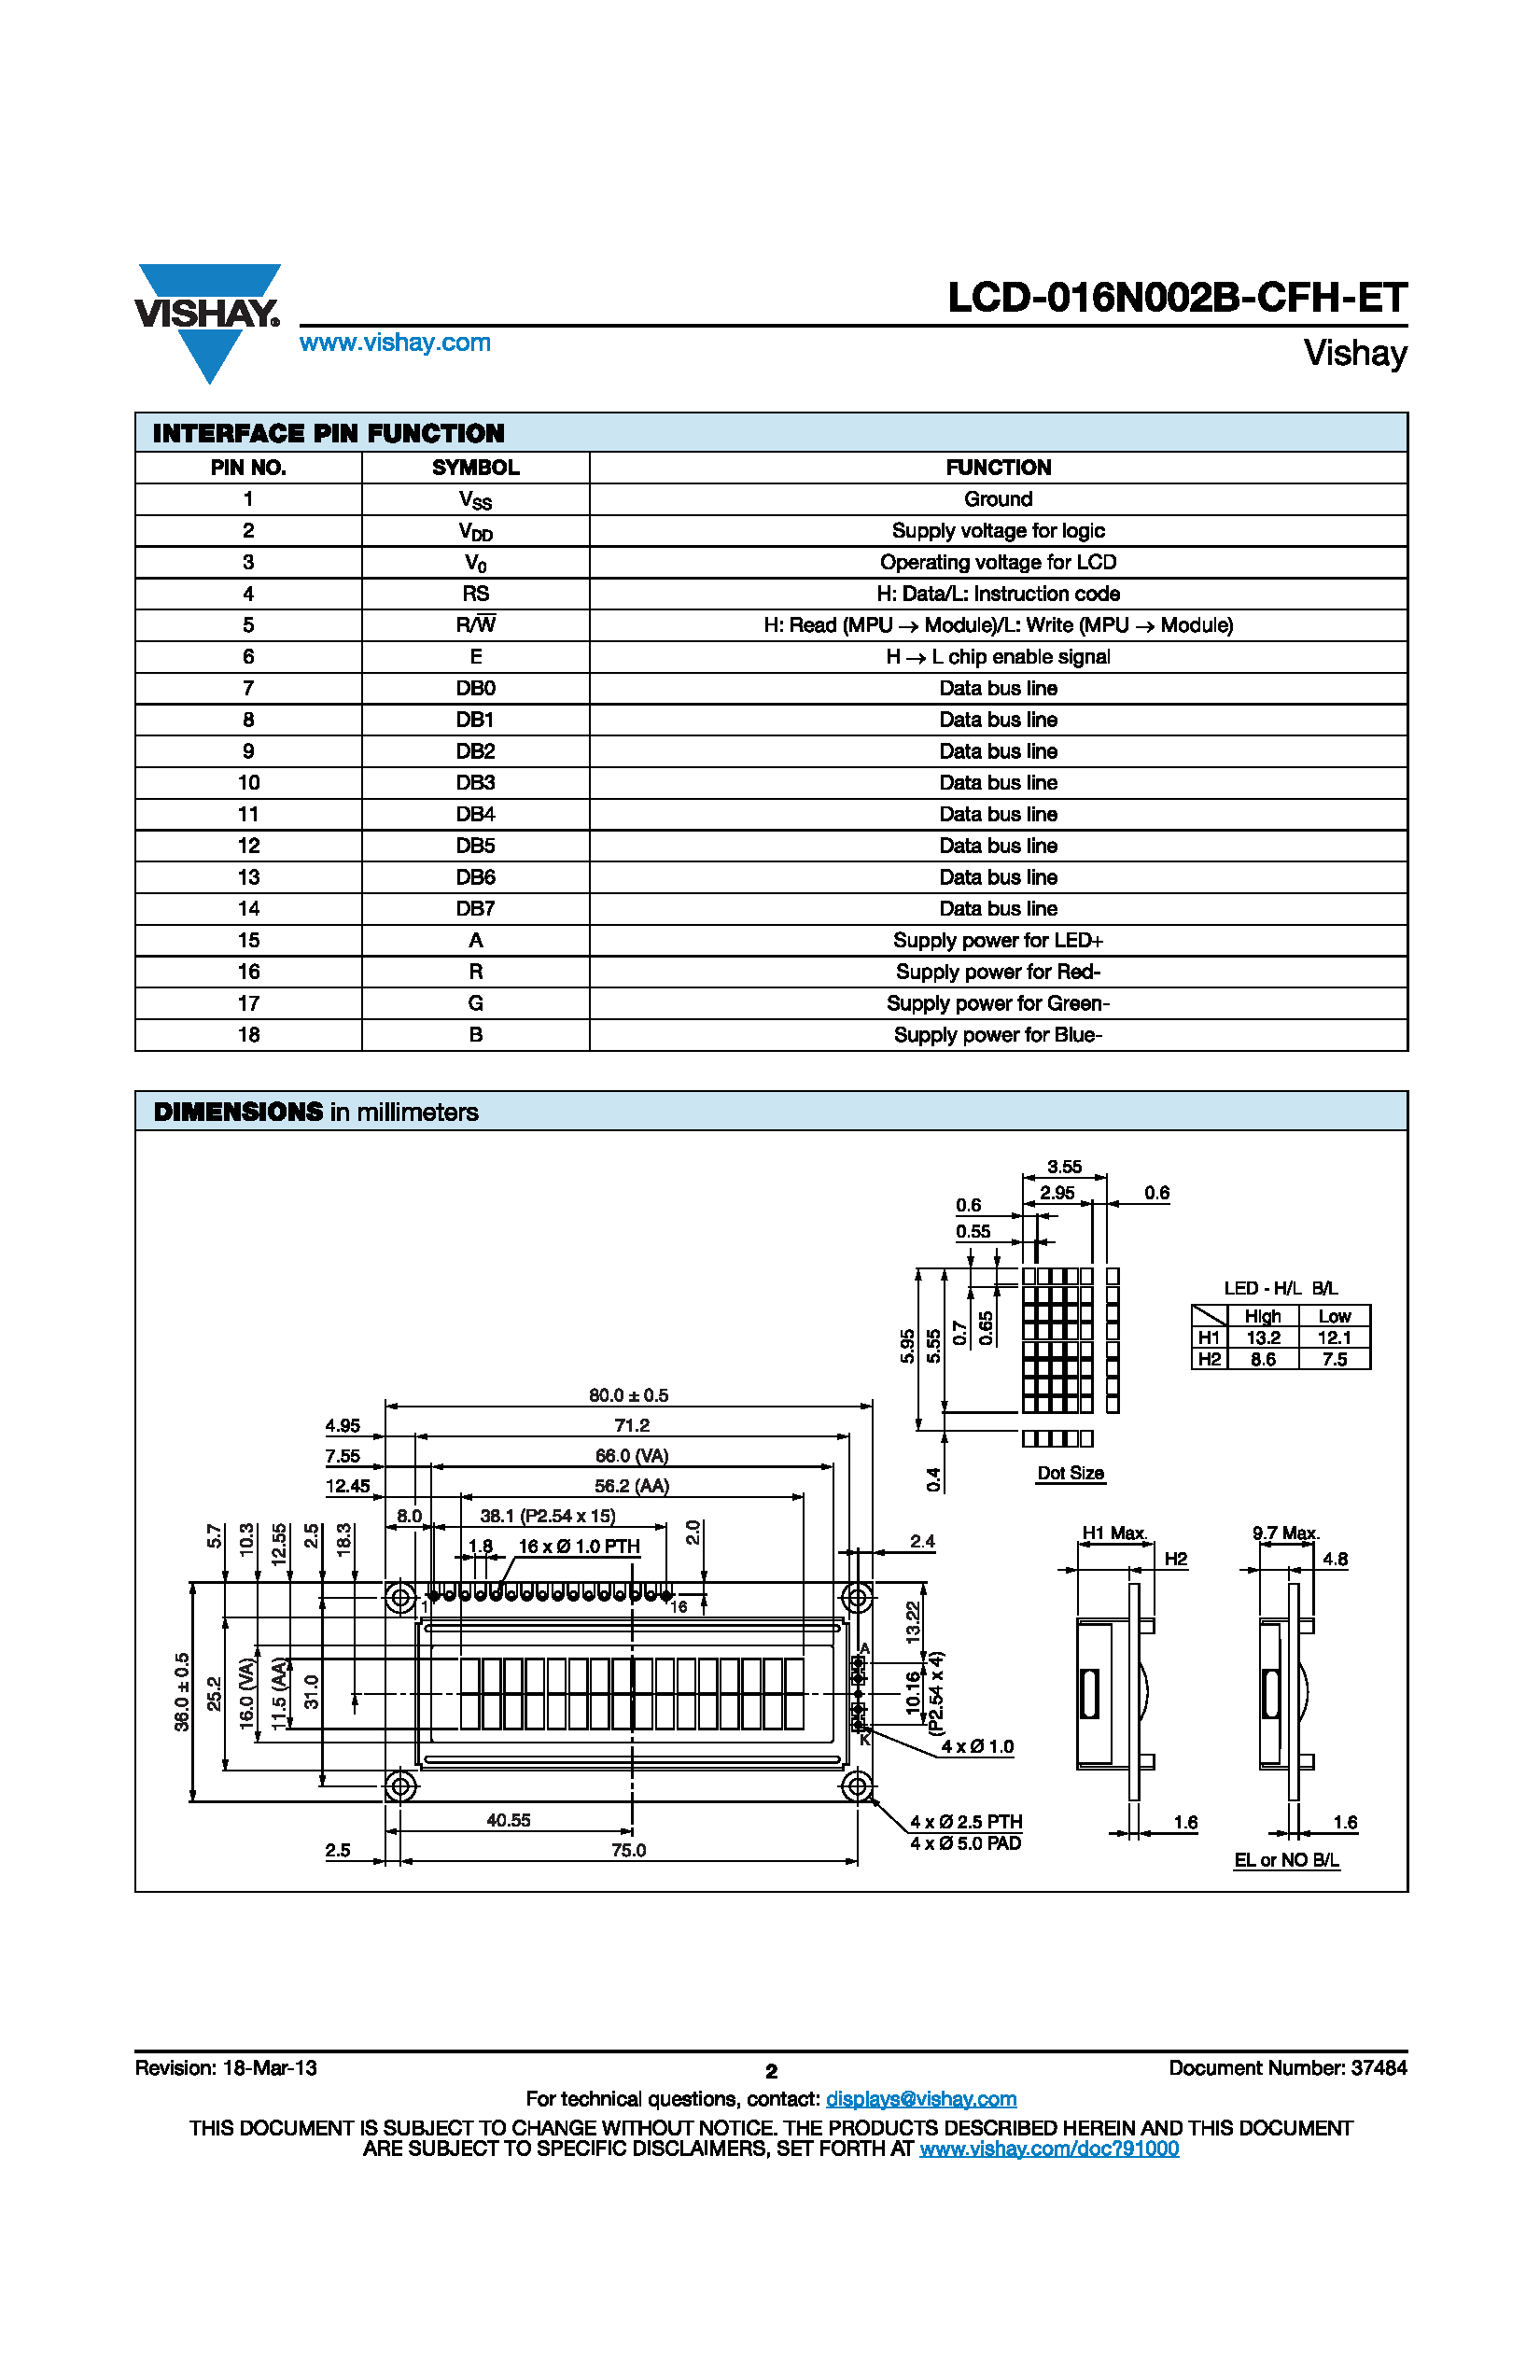
\includegraphics[trim = {30mm 65mm 90mm 250mm},clip,scale=0.5]{6/Img/lcd-16x2.pdf}
        \caption{Esquema LCD de 16x2}
        \label{fig:lcd-16x2-1}
    \end{figure}
    % 
    % 
    \begin{figure}[H]
        \centering
        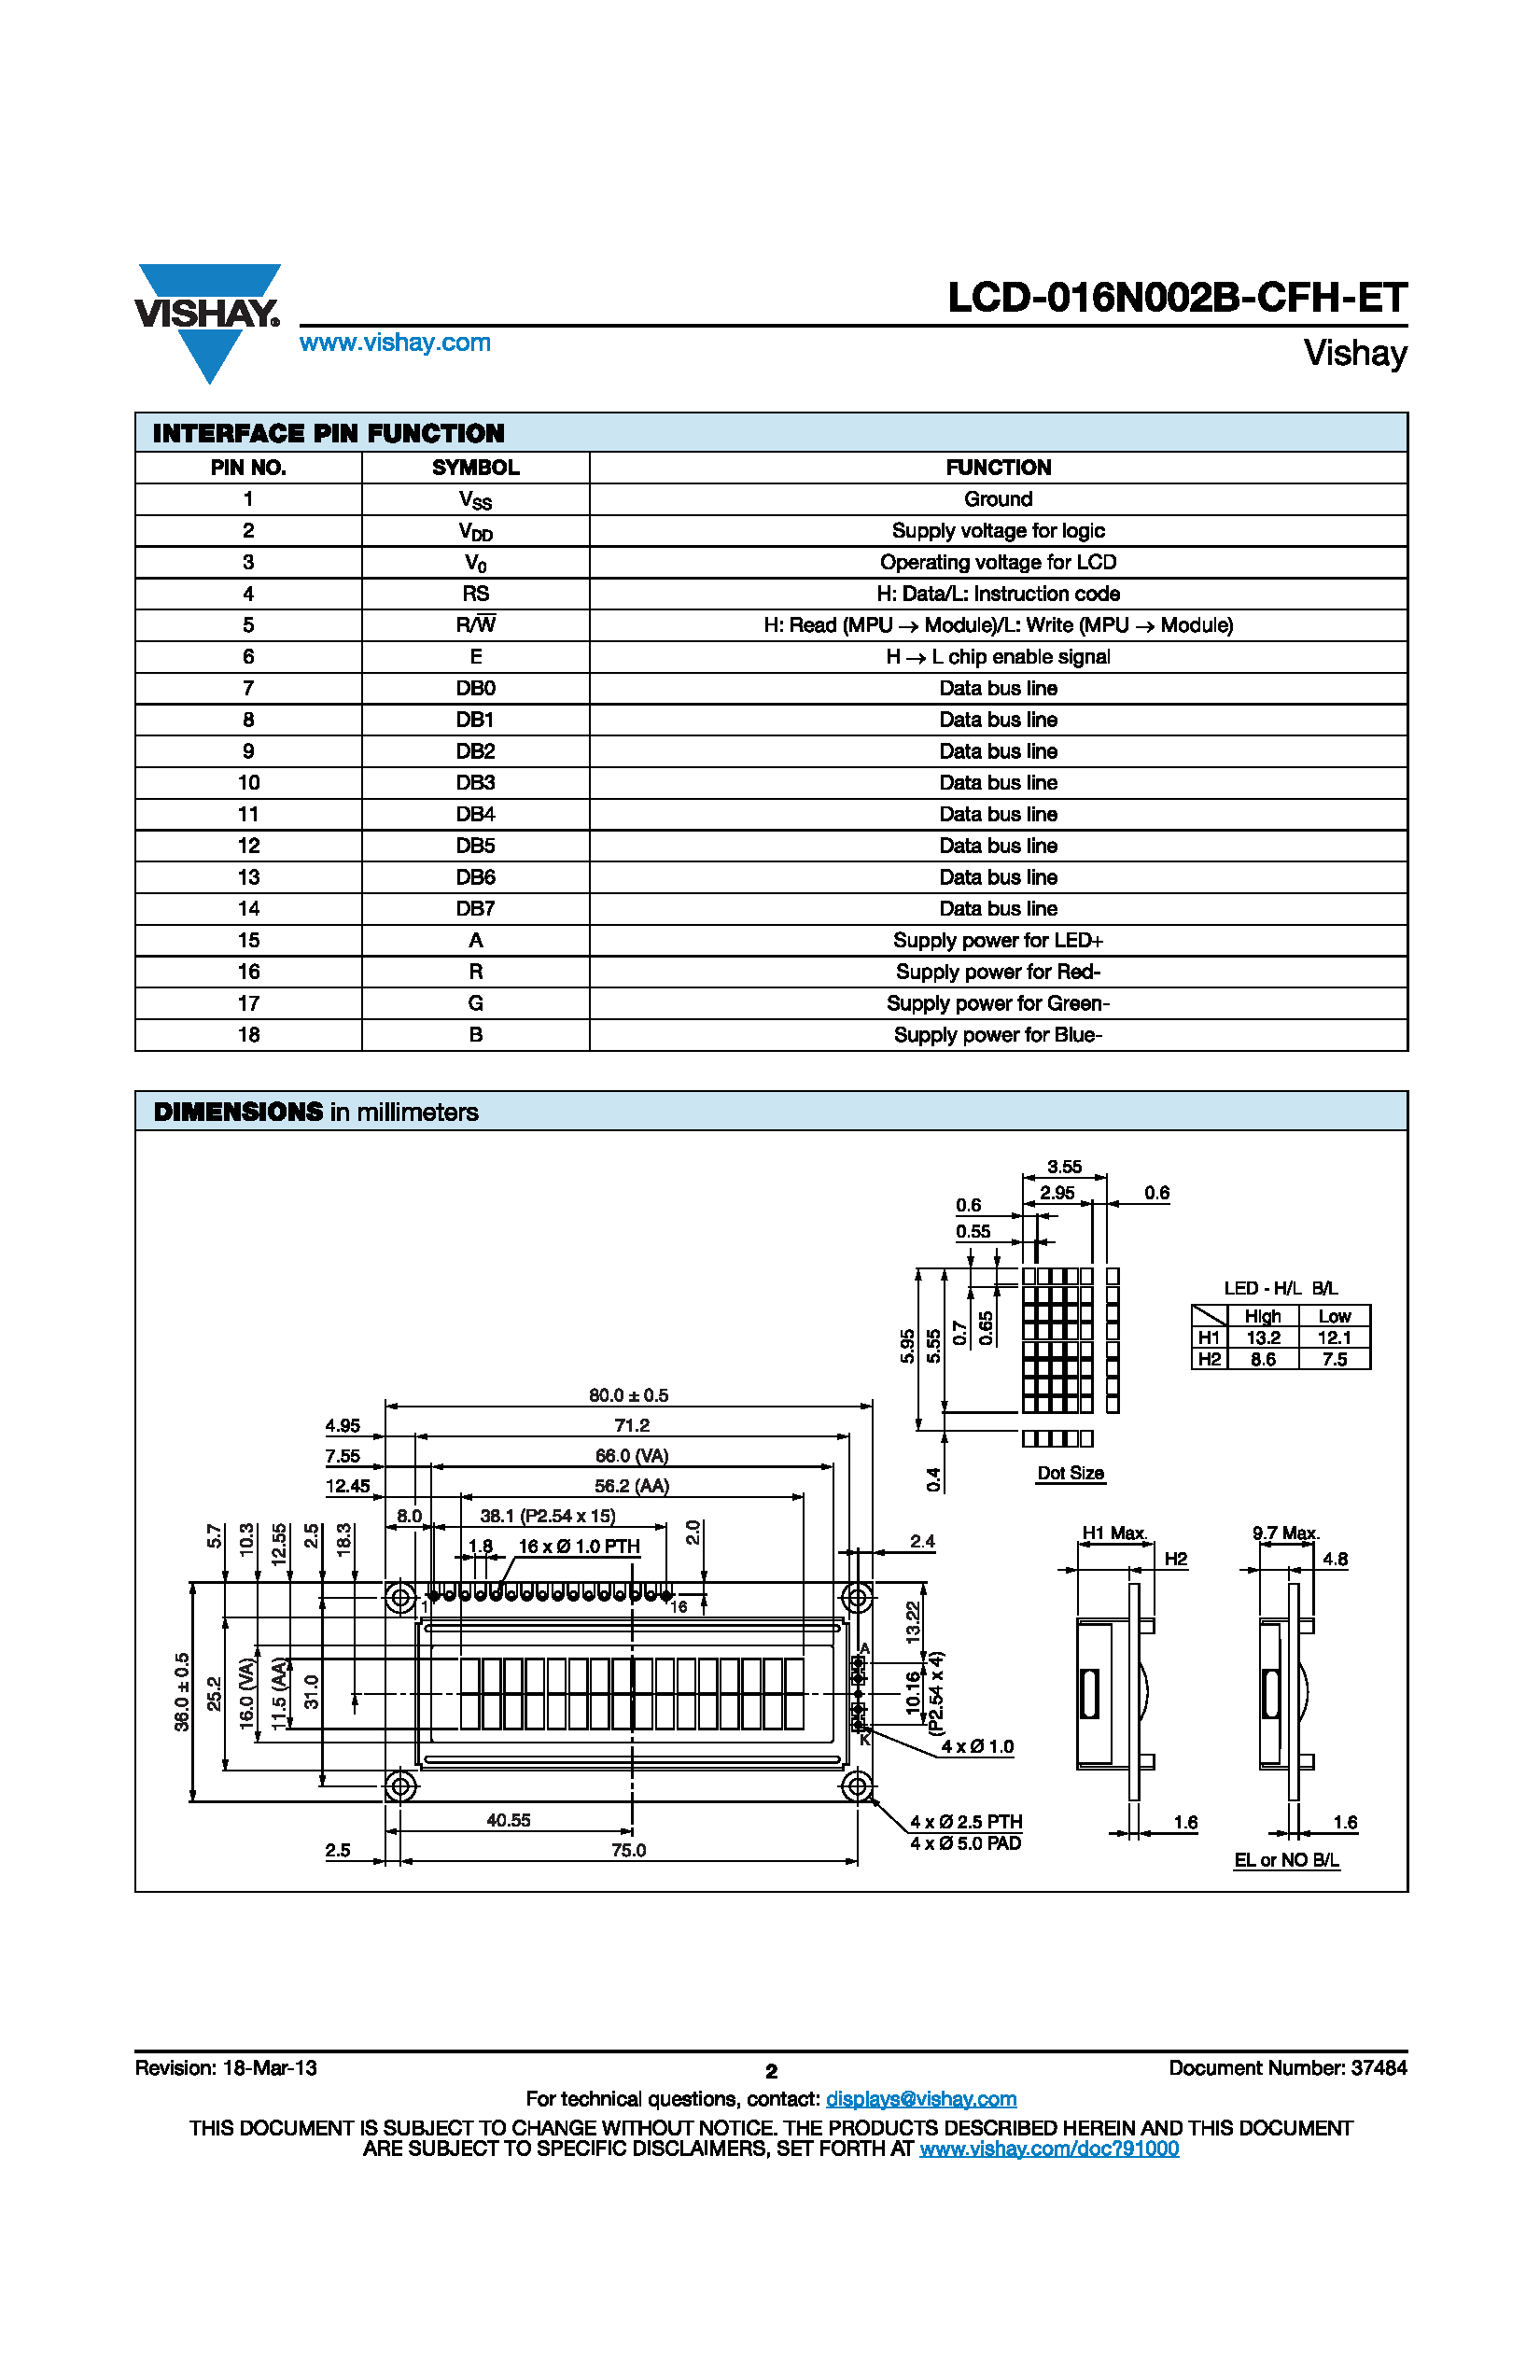
\includegraphics[trim = {30mm 250mm 90mm 20mm},clip,scale=0.5]{6/Img/lcd-16x2.pdf}
        \caption{Esquema LCD de 16x2}
        \label{fig:lcd-16x2-2}
    \end{figure}
    % 
    % 
    \subsection{Prepara tu documento}
    
    Antes de que comiences a utilizar esta plantilla, es recomendable que prepare la información que contendrá en un archivo aparte. 
    Ten preparadas tus gráficas, así como también las tablas aparte, para que sea más fácil integrarlo. 
    Se recomienda fuertemente el uso de \textbf{formato Enhanced Metafile (.emf) para imágenes y gráficas} de resolución óptima. 
    Finalmente, completa y organiza el contenido antes de darle el formato de esta plantilla. 
    
    \subsection{Acrónimos y Abreviaciones}
    
    Los acrónimos y abreviaciones deberán ser definidos únicamente la primera vez que aparecen en el texto, esto para que el lector entienda lo que significan.
    
    \subsection{Ecuaciones}
    
    Las ecuaciones son una excepción a las especificaciones prescritas de esta plantilla. 
    Deberá determinar si su ecuación debe escribirse o no utilizando la fuente Adobe Devangari. 
    Para crear ecuaciones multinivel, puede ser necesario tratar la ecuación como un gráfico e insertarla en el texto después de aplicar el estilo de la platilla.
    Las ecuaciones serán enumeradas de manera consecutiva, y el número de ecuación, entre paréntesis, se colocan al ras de la derecha, utilizando una tabulación derecha. 
    
    \begin{equation}
        \label{eq1}
        x + y = z 
    \end{equation}
    
    Es importante asegurarse de que los símbolos de la ecuación sean definidos antes o inmediatamente después de la ecuación. Utilice “(1)”, en vez de “Eq. 1” al enumerar las ecuaciones, excepto al principio de una oración: “La ecuación (\ref{eq1}) es…”
    
    \section{Resultados y discusión}
    
    Antes de comenzar a preparar tu artículo, es importante que lea primero la guía del autor, la cual incluye los temas o apartados que son necesarios para tener tu trabajo completo.
    Una vez completada la edición del texto, el documento está listo para el uso de esta plantilla. En este archivo recién creado, resalte todo el contenido e importe el archivo de texto preparado. Ahora esta listo para estilizar su documento.
    En esta sección se deben presentar todo lo obtenido de la sección 2, incluidas deducciones o efectos del desarrollo. También se podrán incluir subsecciones numeradas de la siguiente forma:
    
    \subsection{Autores y Afiliaciones}
    
    Para distinguir las afiliaciones de los autores, utilice superíndices iniciando con el número 1, 2, etc., sucesivamente, esto dependerá de la cantidad de los departamentos a los que estén afiliados los autores. En caso de que todos los autores pertenezcan a una mismo departamento e institución, utilizar sólo el superíndice 1. 
    
    \subsection{Identificar los encabezados}
    
    Se les recuerda a los autores que los encabezados deben de estar conforme los solicita la guía del autor. De ahí se puede adaptar el trabajo para que sea más fácil de entender para el lector.
    Los encabezados organizan los temas sobre una base relacional y jerárquica. Por ejemplo, el título del documento es encabezado del texto principal porque todo el material posterior se relaciona y elabora sobre este tema. 
    
    \subsection{Tablas y Figuras}
    
    \begin{enumerate}
        \item Posición de las tablas y figuras: Coloque las figuras y las tablas en la parte superior e inferior de las columnas. Evite colocarlos en medio. Las figuras y las tablas grandes pueden abarcar ambas columnas. Los títulos de las figuras deben de estar debajo de las mismas; los títulos de las tablas deben aparecer encima de ellas. Insértese las figuras y los cuadros después de citarse en el texto. Utilice la abreviatura “Fig. 1”, incluso al principio de una oración. 
    \end{enumerate}
    
    \section{Conclusiones}
    
    Se describe aquí el alcance del trabajo, logros obtenidos y perspectivas para el futuro de este. Se sugiere colocar información cuantitativa obtenida.
    
    \section{Agradecimientos}
    
    Es importante darles su debido reconocimiento a los laboratorios, instituciones, organizaciones, entre otros que han sido participes para la culminación de este trabajo. También es importante mencionar, fondos, proyectos, becas, entre otros que se le han otorgado al o los autores para realizar el trabajo de investigación. Ejemplo: “Los autores agradecen al Concejo Nacional de Ciencia y Tecnología por los recursos otorgados…”
    \section*{Referencias}
    % Ejemplo
    %  @Article{article,
    % 	author = "Author1 LastName1 and Author2 LastName2 and Author3 LastName3",
    % 	title = "Article Title",
    % 	volume = "30",
    % 	number = "30",
    % 	pages = "10127-10134",
    % 	year = "2013",
    % 	doi = "10.3389/fnins.2013.12345",
    % 	URL = "http://www.frontiersin.org/Journal/10.3389/fnins.2013.12345/abstract",
    % 	journal = "Frontiers in Neuroscience"
    % }
    
    % @book{book,
    %   author    = {Author Name}, 
    %   title     = {The title of the work},
    %   publisher = {The name of the publisher},
    %   address   = {The city},
    %   year      = 1993,
    % }
    
    % @incollection{chapter,
    %   author       = {Bauthor Surname}, 
    %   title        = {The title of the work},
    %   editor       = {Editor Name},
    %   booktitle    = {The title of the book},
    %   publisher    = {The name of the publisher},
    %   address      = {The city},
    %   year         = 2002,
    %   pages        = {201-213},
    % }
    
    % @InProceedings{conference,
    %   author = {Cauthor Name and Dauthor Surname and Fauthor LastName},
    %   title = {The title of the work},
    %   booktitle = {The title of the conference proceedings},
    %   year = 1996,
    %   publisher = {The name of the publisher},
    %   editor = {Editor Name1 and Editor Name2},
    %   pages = {41-50},
    % }
    
    % @book{cho,
    %   author       = {Gauthor Name1}, 
    %   title        = {The title of the work},
    %   publisher = {Country code and patent number},
    %   address      = {Patent Country},
    %   year = 2013
    % }
    
    % @book{patent,
    %   author    = {Hauthor Surname1}, 
    %   title     = {The title of the work},
    %   publisher = {Patent number},
    %   address   = {Patent country},
    %   year      = 2010,
    % }
    
    % % please use misc for datasets
    % @misc{dataset, 
    % 	author = "Author1 LastName1 and Author2 LastName2 and Author3 LastName3",
    % 	title = "Data Title",
    % 	year = "2011",
    % 	doi = "10.000/55555",
    % 	URL = "http://www.frontiersin.org/",
    % }
    
    \bibliographystyle{ieeetr}
    \bibliography{26/referencias}
    % 
    % 
    %%%%%%%%%%%%%%%%%%%%%%%%%%%%%%%%%%
    \appendix
    %%%%%%%%%%%%%%%%%%%%%%%%%%%%%%%%%%
    \centering{\section[\appendixautorefname{}]{APÉNDICE}}
    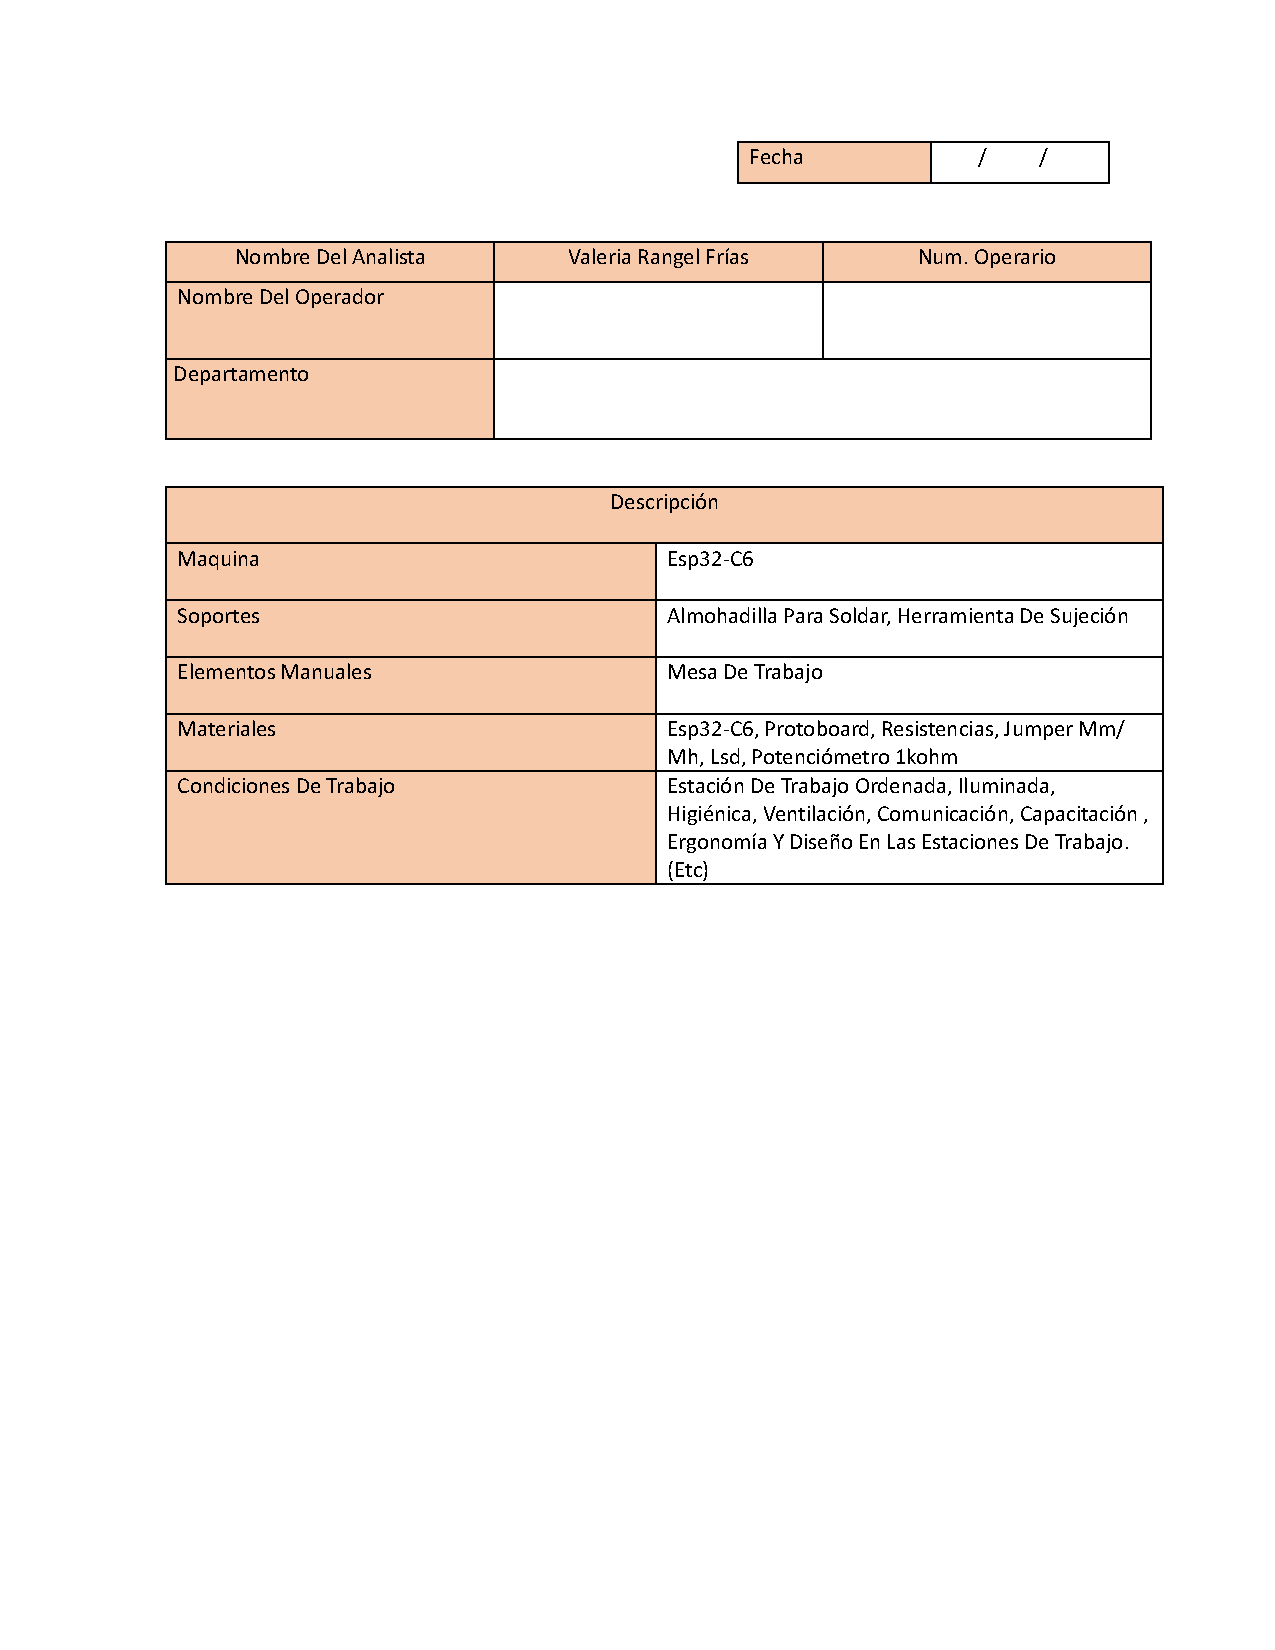
\includepdf[pages=-]{26/Img/camelCase.pdf}\label{anexo:1}
    %%%%%%%%%%%%%%%%%%%%%%%%%%%%%%%%%%%%%%%%
    \centering{\section[\appendixautorefname{}]{APÉNDICE}}
    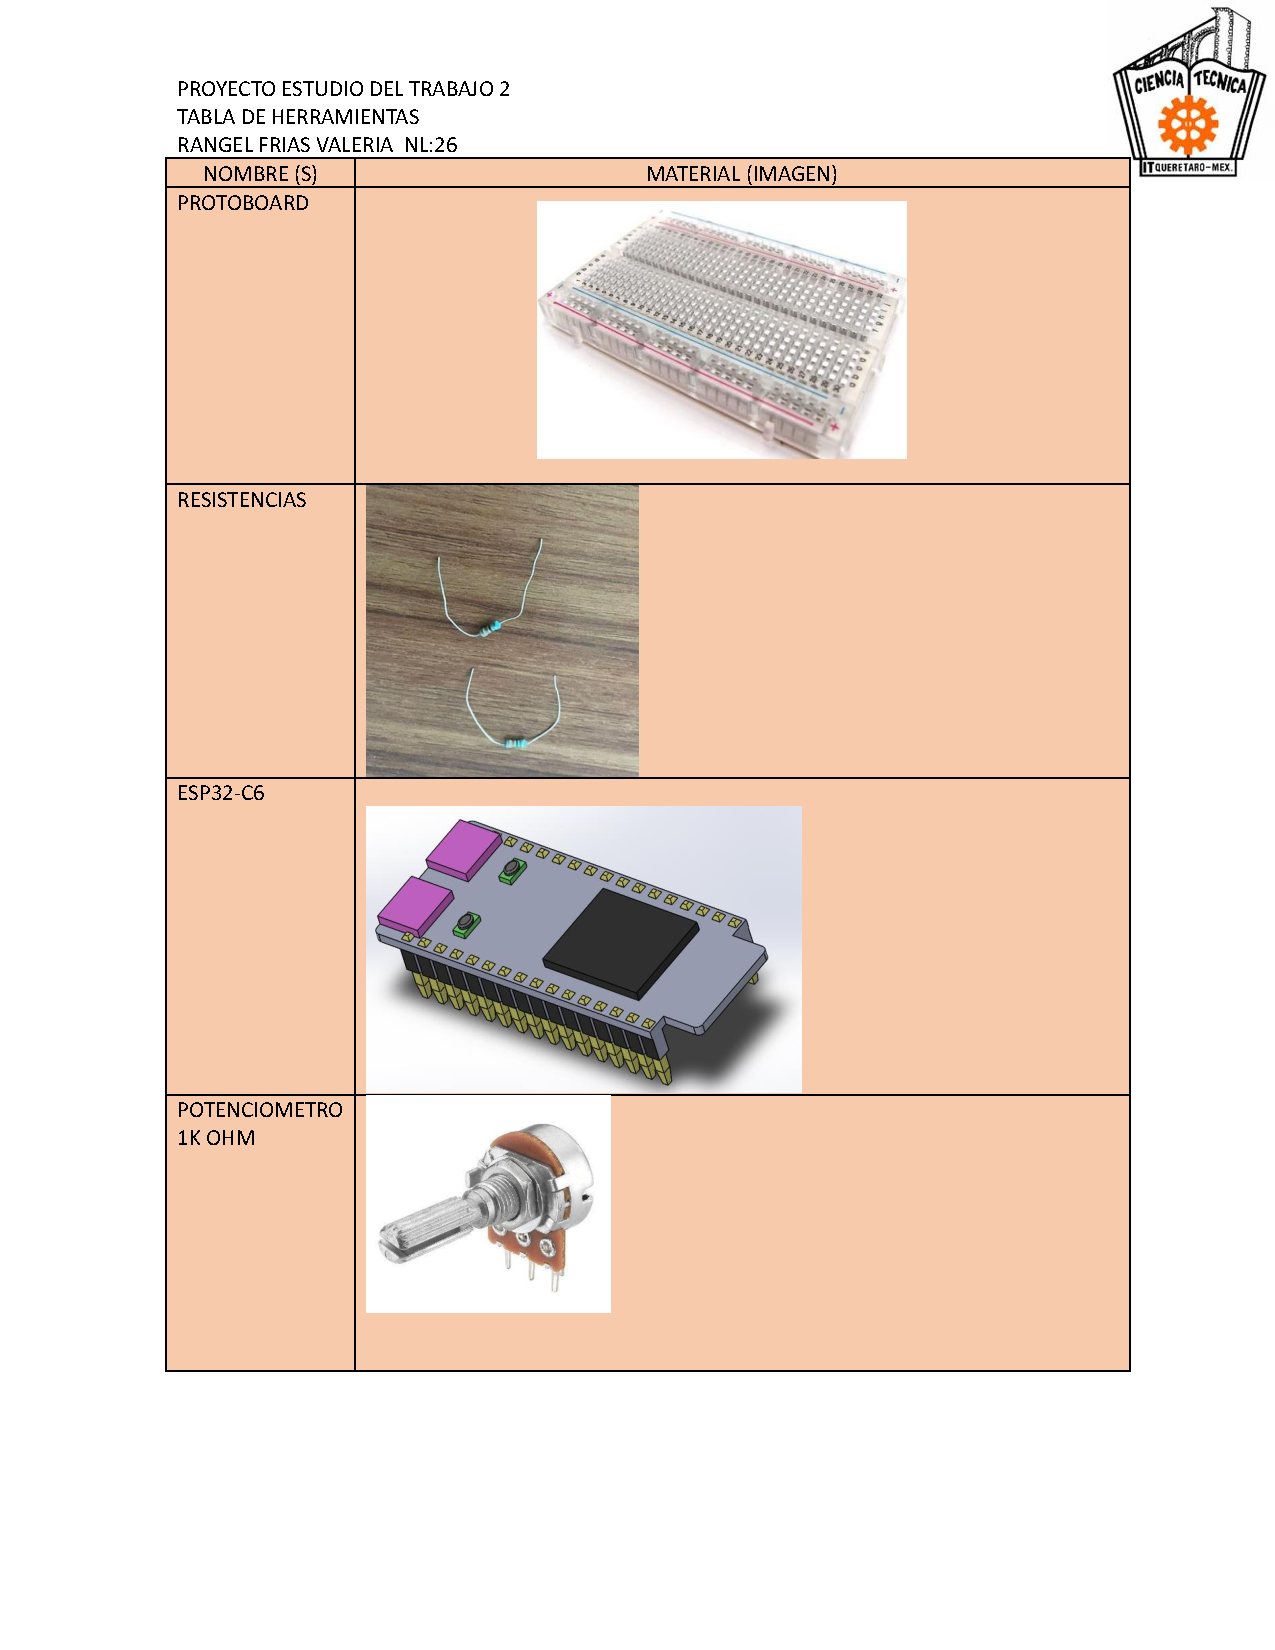
\includepdf[pages=-]{26/Img/camelCase2.pdf}\label{anexo:2}
    %%%%%%%%%%%%%%%%%%%%%%%%%%%%%%%%%%%%%%%%
    \centering{\section[\appendixautorefname{}]{APÉNDICE}}
    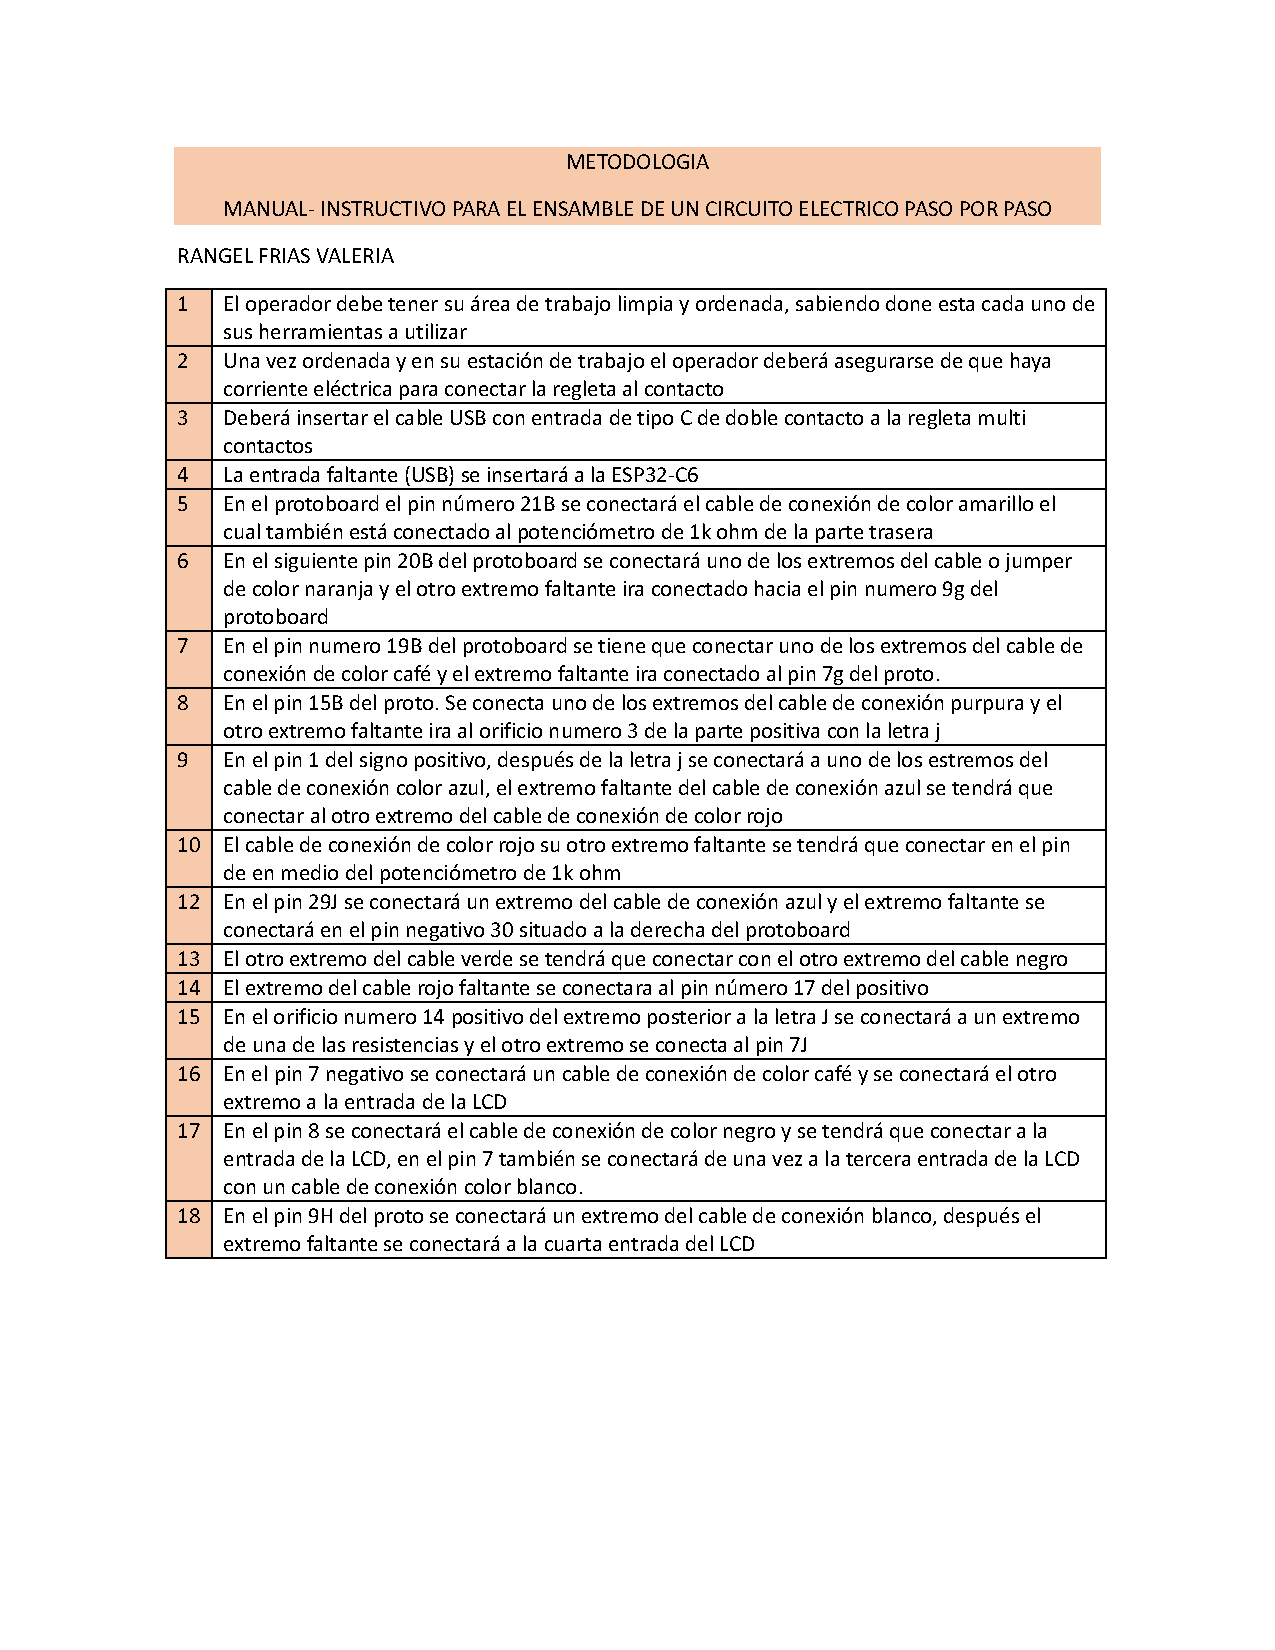
\includepdf[pages=-]{26/Img/camelCase3.pdf}\label{anexo:3}
    %%%%%%%%%%%%%%%%%%%%%%%%%%%%%%%%%%%%%%%%
    